% 三矢量的混合积

\pentry{矢量的叉乘\upref{Cross}}
我们定义以下运算
\begin{equation}
\vec A \cross \vec B \vdot \vec C
\end{equation}
为矢量 $\vec A, \vec B, \vec C$ 的\bb{混合积}. 混合积满足
\begin{equation}\label{TriVM_eq1}
\vec A \cross \vec B \vdot \vec C = \vec B \cross \vec C \vdot \vec A = \vec C \cross \vec A \vdot \vec B 
\end{equation} 
这个公式可由\autoref{TriVM_fig1} 记忆.
\begin{figure}[ht]
\centering
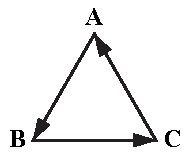
\includegraphics[width=3.2cm]{./figures/TriVM1.pdf}
\caption{\autoref{TriVM_eq1} 记忆法}\label{TriVM_fig1}
\end{figure}
图中箭头的方向由叉乘的方向决定,与点乘无关($\vec A\cross \vec B \vdot \vec C = \vec C \vdot (\vec A \cross \vec B)$).如果混合积的顺序取与箭头相反的方向, 根据叉乘的性质,需要在前面加上负号(叉乘不满足乘法交换律). 下式与上式互为相反数
\begin{equation}
\vec C \cross \vec B \vdot \vec A = \vec B \cross \vec A \vdot \vec C = \vec A \cross \vec C \vdot \vec B
\end{equation} 
另外要注意混合积的方向是由叉乘的顺序所决定的,与点乘的顺序无关.

\subsection{几何法证明}

\begin{figure}[ht]
\centering
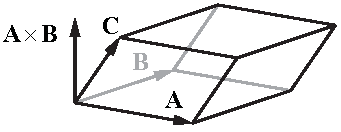
\includegraphics[width=6cm]{./figures/TriVM2.pdf}
\caption{矢量混合积的几何意义} \label{TriVM_fig2}
\end{figure}

如\autoref{TriVM_fig2}, 以三个矢量为棱作平行六面体. 由\autoref{Cross_exe1}\upref{Cross} 可知 $\abs{\vec A \cross \vec B}$ 就是 $\vec A,\vec B$ 所在平行四边形的面积. 令 $\vec A \cross \vec B = \abs{\vec A \cross \vec B} \uvec n$, 则 $\uvec n$ 为平面的法向量, 平行六面体的高为 $\abs{\uvec n \vdot \vec C}$, 所以平行六面体的体积等于底面积乘以高
\begin{equation}
V = \abs{\vec A \cross \vec B} \abs{\uvec n \vdot \vec C} = \abs{\vec A \cross \vec B \vdot \vec C}
\end{equation}
同理可得对于同一平行六面体
\begin{equation}
V = \abs{\vec B \cross \vec C \vdot \vec A} = \abs{\vec C \cross \vec A \vdot \vec B} 
\end{equation}  
这里只证明了\autoref{TriVM_eq1} 的绝对值, 要证明正负号, 定义 $\uvec n \vdot \vec C < 0$ 时 $V$ 为负值即可.

\subsection{代数法证明}
\pentry{行列式\upref{Deter}}
不难证明三矢矢积若展开成分量的形式,等于三个矢量组成的行列式
\begin{equation}
\vec A \cross \vec B \vdot \vec C = \vmat{
A_x & A_y & A_z\\
B_x & B_y & B_z\\
C_x & C_y & C_z}
\end{equation}
而利用行列式中任意两行置换符号改变,即可证明\autoref{TriVM_eq1}.


